\documentclass[18pt]{article}
\usepackage{graphicx}
\usepackage{amsmath}
\graphicspath{{./images/}}
\usepackage{subcaption}

\title{Neural Network and Deep Learning, \\ Micahel Nielsen, Chapter 1 \\Solutions}
\author{Utkarsh Tiwari}
\date{}

\begin{document}

\maketitle

\textbf{Sigmoid neurons simulating perceptrons, part I} \\
Question 1: Suppose we take all the weights and biases in a network of perceptrons, and multiply them by a positive constant, $c>0$
. Show that the behaviour of the network doesn't change. \\ \\
Solution: for perceptrons: $$
output=f(w,x,b)=
\begin{cases}
0 & \text{if } w\cdot x+b \leq 0 \\
1 & \text{if } w\cdot x+b > 0
\end{cases}
$$ 
where $b \equiv -\text{threshold}$,
$w \cdot x \equiv \sum_{j} w_j x_j, \text{ where } w \text{ and } x \text{ are weight and input vectors respectively.}$
\\
After multiplying with a positive constant $c>0$: $$
output=f(w,x,b)=
\begin{cases}
0 & \text{if } cw\cdot x+cb \leq 0 \\
1 & \text{if } cw\cdot x+cb > 0
\end{cases}
$$
$$
=output=f(w,x,b)=
\begin{cases}
0 & \text{if } c(w\cdot x+b) \leq 0 \\
1 & \text{if } c(w\cdot x+b) > 0
\end{cases}
$$
$$
=output=f(w,x,b)=
\begin{cases}
0 & \text{if } (w\cdot x+b) \leq 0 \\
1 & \text{if } (w\cdot x+b) > 0
\end{cases}
$$
\\
\textbf{Q.E.D}
\\

\textbf{Sigmoid neurons simulating perceptrons, part II} \\

Question 2: Suppose we have the same setup as the last problem - a network of perceptrons. Suppose also that the overall input to the network of perceptrons has been chosen. We won't need the actual input value, we just need the input to have been fixed. Suppose the weights and biases are such that $w \cdot x + b \neq 0$
 for the input $x$ to any particular perceptron in the network. Now replace all the perceptrons in the network by sigmoid neurons, and multiply the weights and biases by a positive constant $c>0$
. Show that in the limit as $c \rightarrow \infty$
 the behaviour of this network of sigmoid neurons is exactly the same as the network of perceptrons. How can this fail when $w⋅x+b=0$
 for one of the perceptrons? \\ \\
Solution: For Sigmoid Neurons:
$$
output=f(w,x,b)= \sigma(-w\cdot x-b)
$$ 
where, $$
\sigma(z)=\frac{1}{1 + e^{-z}}
$$
\textbf{Assumption}:
Assume that $x$ is a fixed unknown value where $w \cdot x + b \neq 0$. Then the resulting network will remain unchanged (assuming $c > 0$) as $c \rightarrow \infty$.

\textbf{Case 1}:$$w \cdot x + b < 0:$$\\
$$output=\lim_{c \rightarrow \infty} \frac{1}{1 + e^{c(-w\cdot x-b)}}$$
$$\implies output=\frac{1}{1+e^(\lim_{c \rightarrow \infty}c(-w\cdot x-b)}$$
$$=\frac{1}{1+e^\inf}$$
$$=0$$

\textbf{Case 2}:$$w \cdot x + b > 0:$$\\
$$output=\lim_{c \rightarrow \infty} \frac{1}{1 + e^{c(-w\cdot x-b)}}$$
$$\implies output=\frac{1}{1+e^(\lim_{c \rightarrow \infty}c(-w\cdot x-b)}$$
$$=\frac{1}{1+e^-(\inf)}$$
$$=1$$

This is exactly like a perceptron. \textbf{Q.E.D}

\textbf{Case 3}:$$w \cdot x + b = 0:$$\\
$$output=\lim_{c \rightarrow \infty} \frac{1}{1 + e^{c(-w\cdot x-b)}}$$
$$\implies output=\frac{1}{1+e^(\lim_{c \rightarrow \infty}c(0))}$$
$$=\frac{1}{1+e^0}$$
$$=1/2$$

\textbf{Alternate Approach:}
The sigmoid function (activation function for sigmoid neuron) is a smoothed version of the step function (activation function for perceptron)
\begin{figure}[htbp]
  \centering
  \begin{subfigure}[b]{0.4\textwidth}
    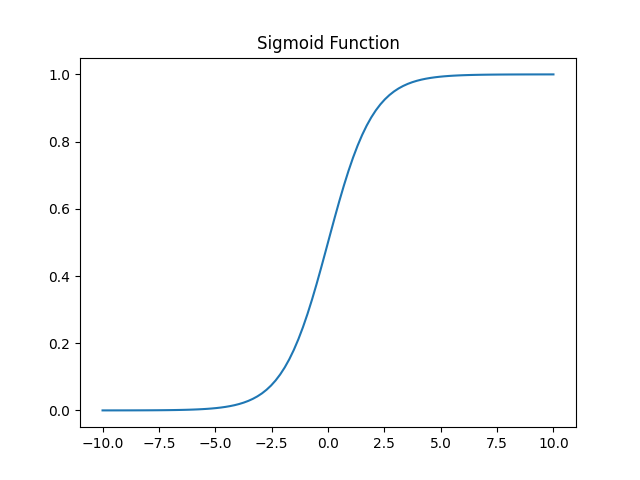
\includegraphics[width=1.3\textwidth]{images/sigmoid.png}
    \caption{Sigmoid Function}
    \label{fig:sigmoid}
  \end{subfigure}
  \hspace{1cm}
  \begin{subfigure}[b]{0.4\textwidth}
    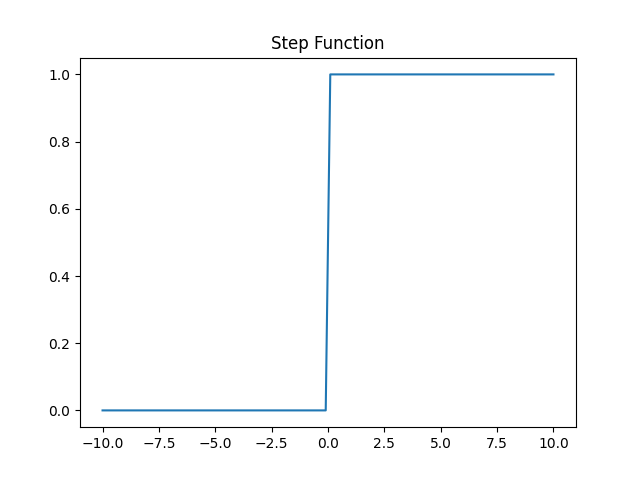
\includegraphics[width=1.3\textwidth]{images/step.png}
    \caption{Step Function}
    \label{fig:step}
  \end{subfigure}
\end{figure}

If the input(s) of the sigmoid function is multiplied by a positive constant $c$ where $c\rightarrow \infty$ then the plot of the sigmoid function starts approaching the shape of the step function.


\begin{figure}[htbp]
    \centering
    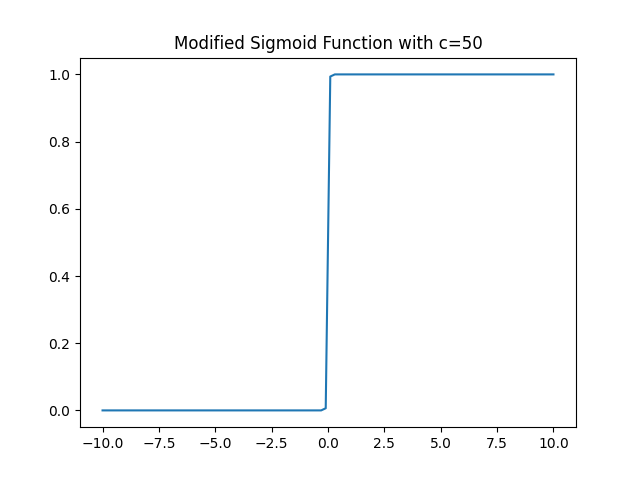
\includegraphics[width=0.7\textwidth]{images/Figure_4.png}
    \caption{Sigmoid Function with c=50 starts resembling the step function. The modified function is $\frac{1}{1+e^(cz)}$}
    \label{fig:my_label}
\end{figure}

So, we can see that as $c \rightarrow \infty$ the activation function on the sigmoid neurons starts resembling the step function. Hence, there is no difference between the two under the given condition. \textbf{Q.E.D}\\
Also, because the step function is undefined for $x=0$ we cannot comment whether the above proved statement holds when $w\cdot x + b = 0$.
\\

\textbf{Question 3, Architecture:}\\
Question: There is a way of determining the bitwise representation of a digit by adding an extra layer to the three-layer network above. The extra layer converts the output from the previous layer into a binary representation, as illustrated in the figure below. Find a set of weights and biases for the new output layer. Assume that the first 3
 layers of neurons are such that the correct output in the third layer (i.e., the old output layer) has activation at least 0.99
, and incorrect outputs have activation less than 0.01
\begin{figure}[htbp]
    \centering
    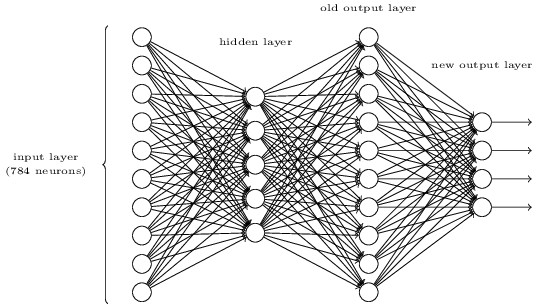
\includegraphics[width=0.9\textwidth]{images/arch_ex.png}
    \label{fig:my_label}
\end{figure}
\\
\\
Solution: We are dealing with conversions from base 10 to base 2 values. The motivation behind this comes from the fact that if the output neurons correspond to binary bits instead of decimal digits we could get upto 10 possible digits $(0_{10}$ to $9_{10})$ using only 4 output neurons.\\
The first node could classify whether the number is even or odd respectively, i.e., it denotes whether the last bit is 0 or 1 (convince youself this is true). A bias in this case in unnecessary because $w\cdot x$ will either be 0 or 1. Hence the weights for the first neuron are:
$$w_9=1$$
$$w_8=0$$
$$w_7=1$$
$$w_6=0$$
$$w_5=1$$
$$w_4=0$$
$$w_3=1$$
$$w_2=0$$
$$w_1=1$$

Which is to say that the neuron outputs 0 for even numbers, and 1 for odd numbers.

Similarly the second neuron (denoting the second to rightmost bit) should be 1 only for {2,3,6,7} and so their weights would be 1 while all other weights would be 0.

Similarly the second neuron (denoting the second to leftmost bit) should be 1 only for {4,5,6,7} and so their weights would be 1 while all other weights would be 0.

The last neuron would be 1 only for {8,9}, so their weights should be 1 while all other are 0.

\bigbreak
\textbf{Gradient Descent and learning rate}:

Question 3: 
\begin{quote}
    Indeed, there's even a sense in which gradient descent is the optimal strategy for searching for a minimum. Let's suppose that we're trying to make a move $\Delta v$ in position so as to decrease $C$ as much as possible. This is equivalent to minimizing $\Delta C \approx \nabla C \cdot \Delta v$. We'll constrain the size of the move so that $\|\Delta v\|=\epsilon$ for some small fixed $\epsilon>0$. In other words, we want a move that is a small step of a fixed size, and we're trying to find the movement direction which decreases $C$ as much as possible. It can be proved that the choice of $\Delta v$ which minimizes $\nabla C \cdot \Delta v$ is $\Delta v=-\eta \nabla C$, where $\eta=\epsilon/\|\nabla C\|$ is determined by the size constraint $\|\Delta v\|=\epsilon$. So gradient descent can be viewed as a way of taking small steps in the direction which does the most to immediately decrease $C$.
\end{quote}
Prove the assertion of the last paragraph. Hint: If you're not already familiar with the Cauchy-Schwarz inequality, you may find it helpful to familiarize yourself with it.\\
Solution: \\
Cauchy-Schwarz inequality states that 
for any vectors $\mathbf{u}$ and $\mathbf{v}$ in an inner product space, we have
\begin{equation}
    \left|\langle \mathbf{u}, \mathbf{v}\rangle \right| \leq \|\mathbf{u}\| \|\mathbf{v}\|,
\end{equation}
where $\langle \cdot, \cdot \rangle$ denotes the inner product and $\|\cdot\|$ denotes the norm.

Applying Cauchy-Schwarz inequality to $\nabla C$ and $\Delta v$:
\begin{equation}
|\nabla C \cdot \Delta \mathbf{v}| \leq \|\nabla C\| \cdot \|\Delta \mathbf{v}\|
\end{equation}\\
$$\implies
({\nabla C\cdot \Delta v})_{min}=-\|\nabla C\| \cdot \|\Delta \mathbf{v}\|$$
$$=-\|\nabla C\| \cdot \epsilon$$ \\
Hence, we want some value of $\Delta v$ such that$$
({\nabla C\cdot \Delta v})=-\|\nabla C\| \cdot \|\Delta \mathbf{v}\|=-\|\nabla C\| \cdot \epsilon
$$
\begin{equation}
({\nabla C\cdot \Delta v})=-\|\nabla C\| \cdot \epsilon
\end{equation}\\
Multiplying each side of (3) by $\nabla C$:

\begin{equation}
\nabla C \cdot ({\nabla C\cdot \Delta v})=-\nabla C \cdot \|\nabla C\| \cdot \epsilon
\end{equation}\\
$$
\|\nabla C\|^2\cdot \Delta v=-\nabla C \cdot \|\nabla C\| \cdot \epsilon
$$\\
$$\implies \Delta v = \frac{-\nabla C \cdot \epsilon}{\|\nabla C\|}$$
\textbf{Q.E.D.}\\ Also, this was such a challenging proof, both to think of and to write in \LaTeX\ \\


The other exercises are trivial (not) and are left as an exercise to the reader (the author is too lazy)\\

Question 4: I explained gradient descent when $C$
 is a function of two variables, and when it's a function of more than two variables. What happens when $C$
 is a function of just one variable? Can you provide a geometric interpretation of what gradient descent is doing in the one-dimensional case?\\

 Question 5: An extreme version of gradient descent is to use a mini-batch size of just 1. That is, given a training input, $x$, we update our weights and biases according to the rules $w_k \rightarrow w'_k = w_k - \eta \frac{\partial C_x}{\partial w_k}$ and $b_l \rightarrow b'_l = b_l - \eta \frac{\partial C_x}{\partial b_l}$. Then we choose another training input, and update the weights and biases again. And so on, repeatedly. This procedure is known as online, on-line, or incremental learning. In online learning, a neural network learns from just one training input at a time (just as human beings do). Name one advantage and one disadvantage of online learning, compared to stochastic gradient descent with a mini-batch size of, say, 20
\end{document}